\begin{frame}[t]{Did drafted workers return after the war?}
    \hypertarget{app:postwar-return}{}
    \scriptsize
    \centering
    \begin{threeparttable}
    \begin{tabular}{lccc}
        \toprule
        & Basic OLS & Kyoku FE & Section FE \\
        \midrule
        Drafted in 1944 & 0.4215$^{***}$ & 0.4216$^{***}$ & 0.4331$^{***}$ \\
         & (0.0124) & (0.0158) & (0.0169) \\
        \addlinespace
        Drafted return rate & \multicolumn{3}{c}{42.3\%} \\
        Non-drafted exiter return rate & \multicolumn{3}{c}{0.0\%} \\
        \midrule
        Drafted workers & \multicolumn{3}{c}{1,849} \\
        Non-drafted exiters (1944) & \multicolumn{3}{c}{3,794} \\
        Kyoku FE & No & Yes & --- \\
        Section FE & No & No & Yes \\
        Controls (tenure, rank) & Yes & Yes & Yes \\
        \bottomrule
    \end{tabular}
    \begin{tablenotes}[flushleft]
        \tiny
        \item \textit{Notes:} OLS regression. Outcome is an indicator equal to 1 if the worker is observed in any postwar directory (1947--1955). Sample is male workers whose last observed year is 1944 (``exiters''), so both groups left in 1944. ``Drafted'' workers are those flagged as drafted in the 1944 TokyoTo directory; the comparison group left for other reasons. Controls include years of tenure in 1944 and position rank. Standard errors clustered by office. $^{***}p<0.01$, $^{**}p<0.05$, $^{*}p<0.1$.
    \end{tablenotes}
    \end{threeparttable}
\end{frame}

\begin{frame}[t]{When did drafted workers return?}
    \centering
    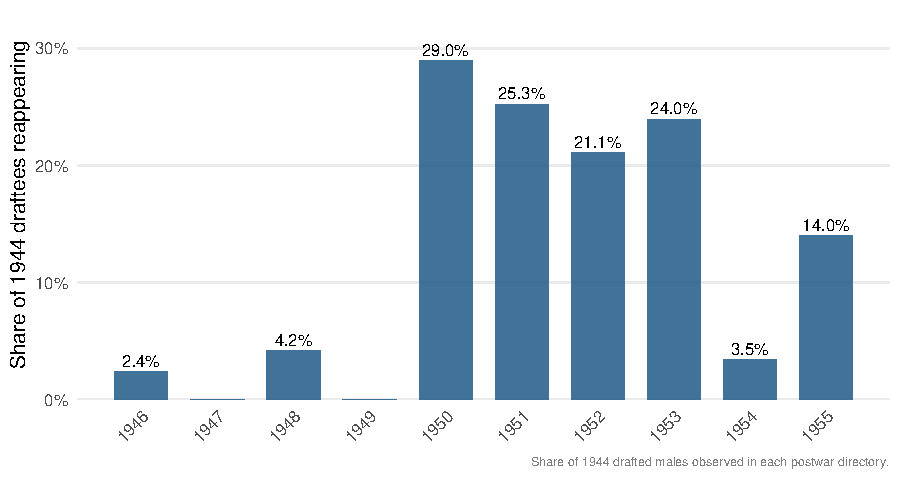
\includegraphics[width=0.84\textwidth]{Results/drafted_postwar_return/drafted_yearly_return_rate.pdf}
    \vspace{1mm}
    \parbox{0.9\textwidth}{\centering\tiny Share of 1944 drafted males (N\,=\,1,849) observed in each postwar Tokyo metropolitan government directory. No 1947 or 1949 directories available. The large spike in 1950 likely reflects the completion of demobilization and occupation-era restructuring.}
\end{frame}

